\documentclass[11pt,journal]{article}
%\usepackage{hyperref}
%\usepackage[breaklinks]{hyperref}
\usepackage{breakurl}
\usepackage{url}
\usepackage{listings}
\usepackage{courier}
\usepackage{amsmath}
%\ifCLASSOPTIONcompsoc
% IEEE Computer Society needs nocompress option
% requires cite.sty v4.0 or later (November 2003)
\usepackage[nocompress]{cite}

\usepackage{graphicx}

\graphicspath{ {D:/Non-game stuff/CS notes/GameTheory/} }

%\else
% normal IEEE
\usepackage{cite}
%\fi

\hyphenation{op-tical net-works semi-conduc-tor}
\addtolength{\oddsidemargin}{-.875in}
\addtolength{\evensidemargin}{-.875in} 
\addtolength{\textwidth}{1.75in}

\addtolength{\topmargin}{-.875in}
\addtolength{\textheight}{1.75in}

\begin{document}
	\title{Algorithmic Game Theory, Assignment 1}
	
	\author{Agata~Borkowska,~UID: 1690550}% <-this % stops a space
		%\protect\\
		%\thanks{}}
	
	% The paper headers



	% IEEEtran.cls defaults to using nonbold math in the Abstract.
	% This preserves the distinction between vectors and scalars. However,
	% if the journal you are submitting to favors bold math in the abstract,
	% then you can use LaTeX's standard command \boldmath at the very start
	% of the abstract to achieve this. Many IEEE journals frown on math
	% in the abstract anyway. In particular, the Computer Society does
	% not want either math or citations to appear in the abstract.
	
	% Note that keywords are not normally used for peerreview papers.
	
	% make the title area
	\maketitle
	
	
	% To allow for easy dual compilation without having to reenter the
	% abstract/keywords data, the \IEEEcompsoctitleabstractindextext text will
	% not be used in maketitle, but will appear (i.e., to be "transported")
	% here as \IEEEdisplaynotcompsoctitleabstractindextext when compsoc mode
	% is not selected <OR> if conference mode is selected - because compsoc
	% conference papers position the abstract like regular (non-compsoc)
	% papers do!
	%\IEEEdisplaynotcompsoctitleabstractindextext
	% \IEEEdisplaynotcompsoctitleabstractindextext has no effect when using
	% compsoc under a non-conference mode.
	
	
	% For peer review papers, you can put extra information on the cover
	% page as needed:
	% \ifCLASSOPTIONpeerreview
	% \begin{center} \bfseries EDICS Category: 3-BBND \end{center}
	% \fi
	%
	% For peerreview papers, this IEEEtran command inserts a page break and
	% creates the second title. It will be ignored for other modes.
	%\IEEEpeerreviewmaketitle
	
	
	
	\section{}
	Note: here we use notation (x,y) to mean that the payoff for player I for the given strategy is x, and the payoff for player II is y. (LateX didn't want to cooperate)
	
	We are presented with the following payoff matrix
	\begin{table}[h]
		\centering
		\begin{tabular}{c|c|c|}
			
			& swerve & straight \\
			\hline
			swerve &(0, 0) & (-2, 2) \\
			\hline
			straight & (2, -2) & (-30, -10) \\
			\hline
		\end{tabular}
	\end{table}
	
	Then for Player 1:
	\[0 \cdot z_{11} + (-2)\cdot z_{12} \geq 2\cdot z_{11} + (-30) \cdot z_{12}  \]
	\[ 2 \cdot z_{21} + (-30) \cdot z_{22} \geq 0 \cdot z_{21} + (-2) \cdot z_{22}  \]
	
	And for Player 2:
	\[ 0 \cdot z_{11} + (-2) \cdot z_{21} \geq 2 \cdot z_{11} + (-10) \cdot z_{21}  \]
	\[ 2 \cdot z_{12} + (-10) \cdot z_{22} \geq 0 \cdot z_{12} + (-2) \cdot z_{22} \]
	
	With
	\[ z_{11} + z_{12} + z_{21} + z_{22} =1 \]
	\[ z_{11}, z_{12}, z_{21}, z_{22} \geq 0  \]
	
	We can express this as a linear programming problem:
	\begin{align*}
		\text{Maximise: } & 0\cdot z_{11} + 0 \cdot z_{12} + 0 \cdot z_{21} + z_{22} &\\
		\text{subject to: } & &\\
		 -&2\cdot z_{11} + 28\cdot z_{12} \geq 0\\
		& 2 \cdot z_{21} - 28 \cdot z_{22}  \geq 0\\
		 -&2 \cdot z_{11} + 8 \cdot z_{21} \geq 0\\
		& 2 \cdot z_{12} -8 \cdot z_{22} \geq 0 \\
	\end{align*}
	
	This gives the following probabilities:
	
	\begin{table}[h]
		\centering
		\begin{tabular}{c|c|c|}
			
			& swerve & straight \\
			\hline
			swerve & 0 & $\frac{4}{19}$ \\
			\hline
			straight & $\frac{14}{19}$ & $\frac{1}{19}$ \\
			\hline
		\end{tabular}
	\end{table}
	And the probability of collision is $\dfrac{1}{19}$. 
	
	To check that this is indeed a correlated equilibrium, we substitute the values into the inequalities:
	
	\begin{align*}
		0 - 2\cdot \dfrac{4}{19} \geq 0 - 30 \cdot \dfrac{4}{19}  &\Longrightarrow -2 \cdot \dfrac{4}{19} \geq -30 \cdot \dfrac{4}{19}  \\
		2\cdot \dfrac{14}{19} -30 \cdot \dfrac{1}{19} \geq -2 \cdot \dfrac{1}{19} & \Longrightarrow 2 \cdot \dfrac{14}{19} \geq 28 \cdot \dfrac{1}{19}  \\
		0 - 2 \cdot \dfrac{14}{19}  \geq 2 \cdot 0 - 8 \cdot \dfrac{14}{19} &  \Longrightarrow -2 \cdot \dfrac{14}{19} \geq -8 \cdot \dfrac{14}{19} \\
		2 \cdot \dfrac{4}{19} -10 \cdot \dfrac{1}{19} \geq 0 - 2 \cdot \dfrac{1}{19} & \Longrightarrow 2 \cdot \dfrac{4}{19} \geq 8 \cdot \dfrac{1}{19}  \\
	\end{align*}
	All the inequalities hold, so we have found a correlated equilibrium. 
	%\IEEEPARstart{}{} 
	
	\section{} 
	To demonstrate that for the given auction we can run the VCG mechanism in polynomial time, we will reduce it to the problem of finding a maximal matching in a weighted graph.
	
	First note that each bidder has a valuation for each item, i.e. $v_i(s_j)$ is defined for each bidder $i$ and each item $s_j$. Furthermore for a subset $S'\subseteq S$ of items, containing a $s_j$ valued more than any other item in the set, the value of the subset is equal to the value of $s_j$. Therefore, we may just as well consider only singleton sets. Adding more items to the set will not increase its value.
	
	Now we can represent the auction as a (complete) bipartite graph, with one set of vertices being the bidders, the other set the items. The edges between the two sets will be weighted with the values $v_i(s_j) = v_{ij}$. The graph is shown below, with thick edges showing a matching.
	
	\begin{figure}[h]
		\centering
		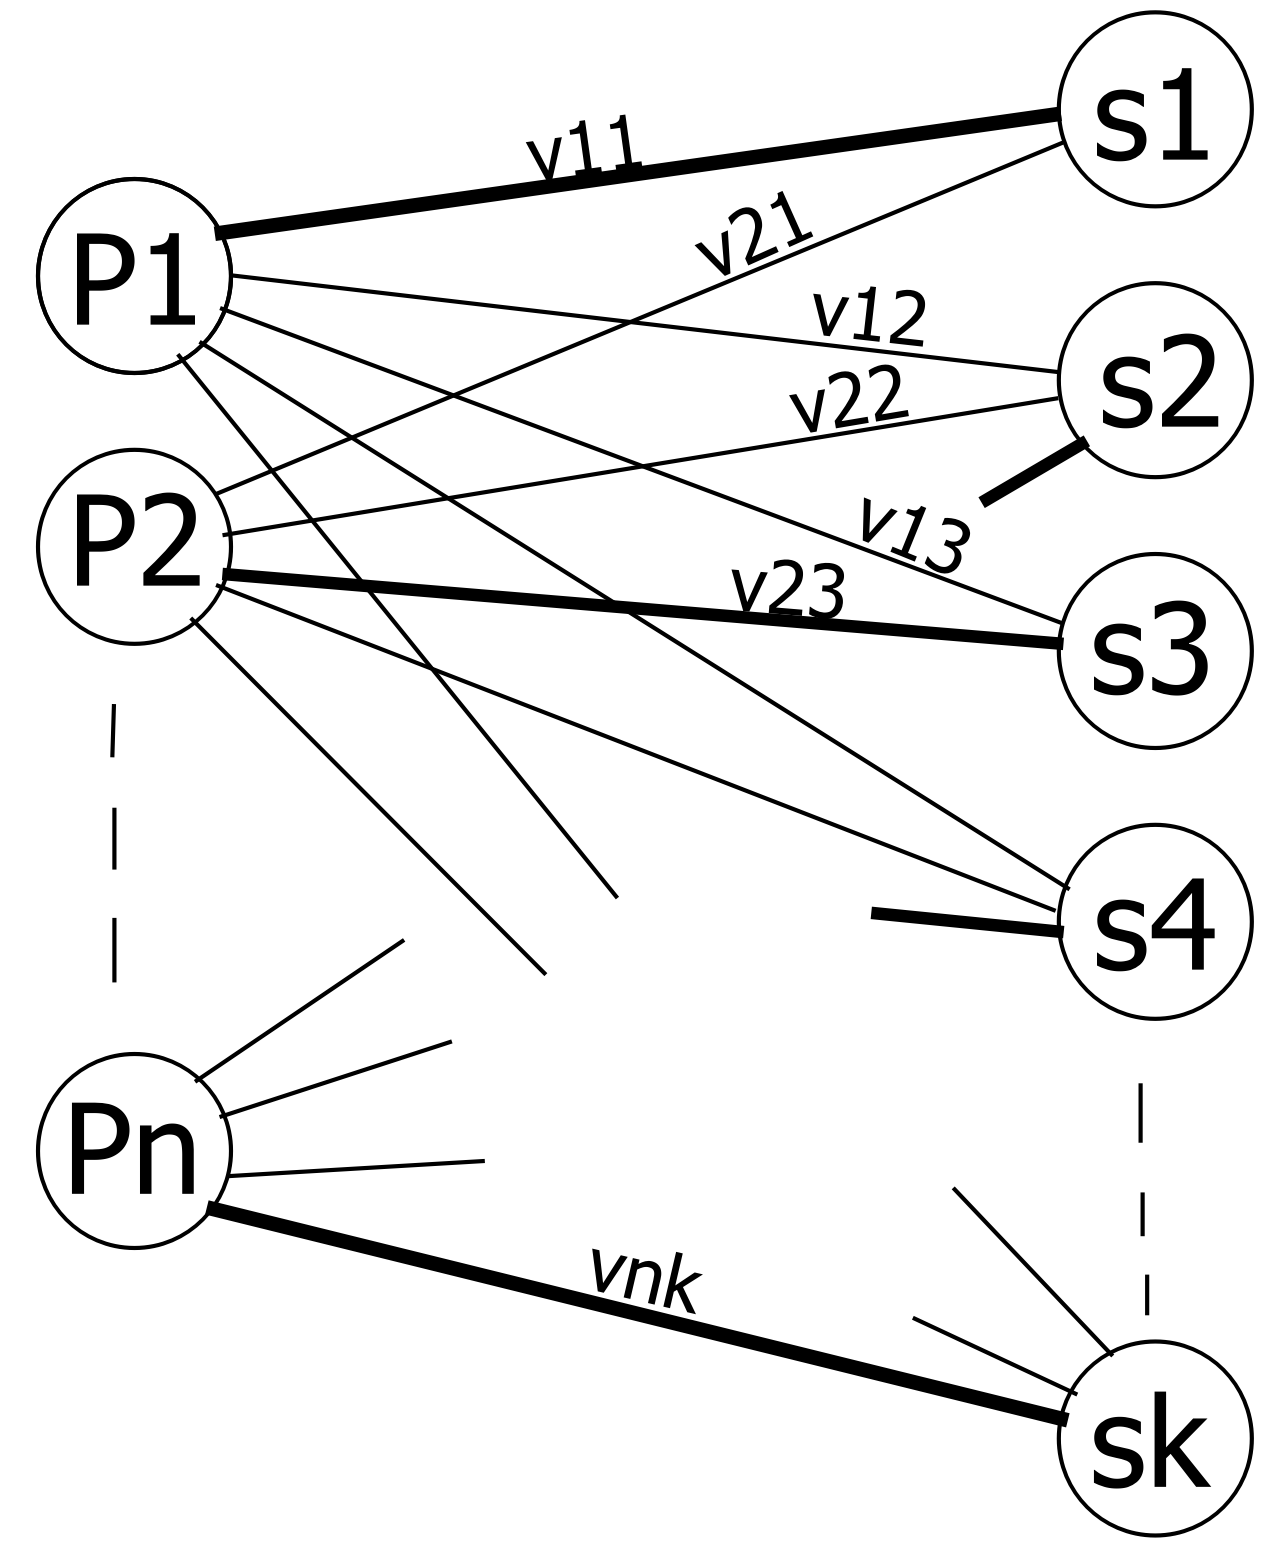
\includegraphics[scale=0.7]{matching.png}
		\caption{Bipartite graph representing the auction}
	\end{figure}
	
	It is of course possible that there will be more bidders than items, in which case some bidders will not get anything out of the auction, or more items than bidders, in which case adding the leftover items to some sets in the allocation will not change the value or the payoff for anyone.

	We can find a matching of maximal weight in polynomial time. We now need to show that this matching will represent an allocation that would be achieved by the VCG mechanism, i.e. an optimal one.
	
	Let us assume bidder i is allocated item $s$ in the matching, while VCG would allocate $s'$. We have two possibilities. Firstly, let us say that the item $s'$ is not allocated to anyone else. Then VCG would give $s'$ to bidder i if and only if $v_i(s') \geq v_i(s)$. If it is strictly greater, then swapping $s$ for $s'$ would increase the value of the matching, contradicting its maximality. If $v_i(s) = v_i(s')$ then the value achieved by the matching is the same as that of the VCG mechanism.
	
	Now let us say that $s'$ given to the bidder i by VCG, is allocated to some other bidder j in the matching. Let us swap the edge $v_i(s)$ for $v_i(s')$ and remove $v_j(s')$. Now j is not allocated any items, so we can give them an item with the highest values, chosen from the set of $s$ and the items not allocated to anyone else. If that item has a value greater than $v_j(s')$, we increase the value of the matching - contradiction.
	
	Therefore VCG will find an alloation with the same value as the maximal matching on the weighted bipartite graph.
	
	\section{}	
	
	Recall that without fixing the opening bid, the expected revenue was the value of the second-highest bid, $x$. It was given by:
	
	\[\int^{1}_{0}x \cdot 2 \cdot (1-x) dx = \dfrac{1}{3}\]
	
	Where $ 2 \cdot (1-x)$ is the probability that two bids are greater or equal to x. It arises in two different ways: we can have bidder 1 bidding x, and bidder 2 submitting a greater bid, probability of which is $f(x)\cdot (1 - F(x)) = 1 - x$, where $f(x)$ is the probability density function and $F(x)$ is the cumulative density function. The other option is with the roles being reversed. Hence we arrive at $2\cdot(1-x)$.
	
	Now consider the scenario where for all $x \leq r$, for some $r \in [0,1]$, the revenue is fixed at r. For all $x \geq r$ the revenue is as before. When one player bids below r, and the other above, the probability of that is $2\cdot f(x)\cdot(1 - F(r))$. Otherwise the revenue is 0.
	
	Therefore, the expected revenue is given by:
	
	\[\int^{1}_{r}x \cdot 2 \cdot (1-x) dx + \int^{r}_{0}r\cdot 2\cdot f(x)\cdot(1 - F(r)) dx  \]
	\[=\int^{1}_{r}x \cdot 2 \cdot (1-x) dx + \int^{r}_{0}r\cdot 2\cdot (1 - r) dx  \]
	\[= 2 \cdot (\frac{x^2}{2} - \frac{x^3}{x})\Bigr| ^{1}_{r}  + 2\cdot(r - r^2)x \Bigr|_{0}^{r} \]
	\[= \frac{1}{3} - 2(\frac{r^2}{2} - \frac{r^3}{3}) + 2r^2 - 2r^3\]
	\[= \frac{1}{3} + r^2 - \frac{4r^3}{3} \]
	
	This function attains its maximum at  a value of r for which
	\[ \frac{d}{dr} ( \frac{1}{3} + r^2 - \frac{4r^3}{3}  ) = 0  \]
	\[\Rightarrow 2r - 4r^2 = 0 \]
	
	Which is at $r=0$ and $r = \frac{1}{2}$. Plotting the graph, we find that the maximum is at $r=\frac{1}{2}$. 
	
	\begin{figure}[h]
		\centering
		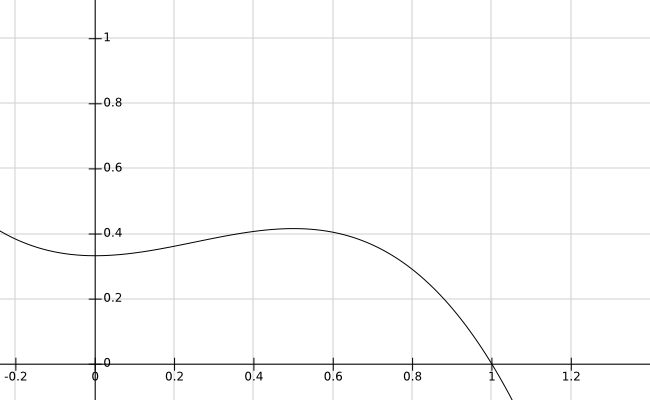
\includegraphics[scale=0.7]{save.png}
		\caption{Plot of the expected revenue function}
	\end{figure}
	
	At this point the expected revenue is $\frac{5}{12}$. Thus it is possible for the auctioneer to have expected revenue greater than $\frac{1}{3}$, and that happens when the value of the opening bid $r$ is $ \frac{1}{2} $.
	

	
	
	% that's all folks
\end{document}

